\let\negmedspace\undefined
\let\negthickspace\undefined
\documentclass[journal]{IEEEtran}
\usepackage[a5paper, margin=10mm, onecolumn]{geometry}
%\usepackage{lmodern} % Ensure lmodern is loaded for pdflatex
\usepackage{tfrupee} % Include tfrupee package

\setlength{\headheight}{1cm} % Set the height of the header box
\setlength{\headsep}{0mm}     % Set the distance between the header box and the top of the text

\usepackage{gvv-book}
\usepackage{gvv}
\usepackage{cite}
\usepackage{amsmath,amssymb,amsfonts,amsthm,mathtools}
\usepackage{algorithmic}
\usepackage{graphicx}
\usepackage{textcomp}
\usepackage{xcolor}
\usepackage{txfonts}
\usepackage{listings}
\usepackage{enumitem}
\usepackage{mathtools}
\usepackage{gensymb}
\usepackage{comment}
\usepackage[breaklinks=true]{hyperref}
\usepackage{tkz-euclide} 
\usepackage{listings}
\def\inputGnumericTable{}                                 
\usepackage[latin1]{inputenc}                                
\usepackage{color}                                            
\usepackage{array}                                            
\usepackage{longtable}                                       
\usepackage{calc}                                             
\usepackage{multirow}                                         
\usepackage{hhline}                                           
\usepackage{ifthen}                                           
\usepackage{lscape}
\begin{document}

\bibliographystyle{IEEEtran}
\vspace{3cm}

\title{4.3.2}
\author{EE24BTECH11002 - Agamjot Singh}
% \maketitle
% \newpage
% \bigskip
{\let\newpage\relax\maketitle}

\renewcommand{\thefigure}{\theenumi}
\renewcommand{\thetable}{\theenumi}
\setlength{\intextsep}{10pt} % Space between text and floats

\textbf{Question:}
\newline
Find the equation of the line passing through $\myvec{0\\0}$ with slope $m$.
\newline
\textbf{Solution:}
\newline

\begin{table}[h!]    
	\centering
	\begin{tabular}[12pt]{ |c| c|}
    \hline
    \textbf{Variable} & \textbf{Description}\\ 
    \hline
	$\vec{A}$ & Point to be found\\
    \hline
	$\vec{B}$ & $(0, 0)$ point\\
    \hline
	$\vec{C}$ & $(6, 0)$ point\\
    \hline
	$\vec{\angle \vec{ABC}}$ & $60 \degree$\\ 
    \hline
    \end{tabular}
	\caption{Variables Used}
	\label{tab4-4.3.2}
\end{table}

Let $\vec{n}$ be the normal vector to the given line.
\begin{align}
	\vec{n} = \myvec{-m\\1}
\end{align}
The equation for the line is given by
\begin{align}
	\vec{n}^\top\brak{\vec{x} - \vec{A}} &= 0\\
	\myvec{-m & 1}\brak{\vec{x} - \myvec{0\\0}} &= 0\\
	\implies \myvec{-m & 1}\vec{x} &= 0 
\end{align}

\begin{figure}[h!]
   \centering
   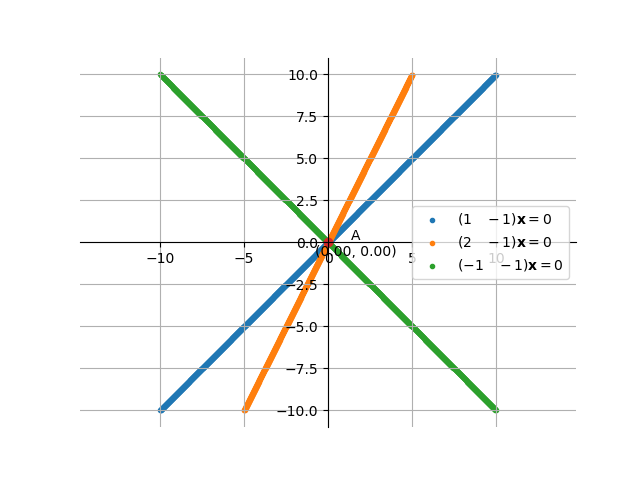
\includegraphics[width=0.7\linewidth]{figs/graph.png}
   \caption{Representing lines with slopes m = 1, 2, -1}
\end{figure}

\end{document}
